% layout and global options
\documentclass
[
  draft    = true,
  fontsize = 11pt,
  parskip  = half-,
  BCOR     = 0pt,
  DIV      = 11,
  ngerman,
  dvipsnames
]
{scrartcl}

% default packages
\usepackage[utf8]{inputenc}
\usepackage[T1]{fontenc}
\usepackage{babel}
\usepackage{lmodern}
% extra packages
\usepackage{amsmath}
\usepackage{amssymb}
\usepackage{graphicx}
\usepackage{tikz}

% enable calculations in TikZ
\usetikzlibrary{calc}

% no headers no footers
\pagestyle{empty}

% ------------------------------------------------------------------------------
\begin{document}
% ------------------------------------------------------------------------------

% -------------------------
\section*{Ableitungsregeln}
% -------------------------
\begin{tabular}{rll}
  Potenzregel:\qquad\qquad
  & $f(x)=x^n$
  & $f'(x)=n\cdot x^{n-1}$
  \\
  & $f(x)=x^3$
  & $f'(x)=3\cdot x^2$
  \\[2ex]
  Faktorregel:\qquad\qquad
  & $f(x)=a\cdot g(x)$
  & $f'(x)=a\cdot g'(x)$
  \\
  & $f(x)=4\cdot x^3$
  & $f'(x)=4\cdot3\cdot x^2=12\cdot x^2$
  \\[2ex]
  Summenregel:\qquad\qquad
  & $f(x)=g(x)+h(x)$
  & $f'(x)=g'(x)+h'(x)$
  \\
  & $f(x)=3\cdot x+x^2$
  & $f'(x)=3+2\cdot x$
  \\[2ex]
  Ableitung einer\phantom{:}\qquad\qquad
  & $f(x)=c$
  & $f'(x)=0$
  \\
  Konstanten:\qquad\qquad & $f(x)=-17$
  & $f'(x)=0$
  \\[2ex]
  Produktregel:\qquad\qquad
  & $f(x)=g(x)\cdot h(x)$
  & $f'(x)=g'(x)\cdot h(x)+g(x)\cdot h'(x)$
  \\
  & $f(x)=x^2\cdot\sin(x)$
  & $f'(x)=2\cdot x\cdot\sin(x)+x^2\cdot\cos(x)$
  \\[4ex]
  Quotientenregel:\qquad\qquad
  & $\displaystyle f(x)=\frac{g(x)}{h(x)}$
  & $\displaystyle f'(x)=\frac{g'(x)\cdot h(x)-g(x)\cdot h'(x)}{\left[g(x)\right]^2}$
  \\[3ex]
  & $\displaystyle f(x)=\frac{x^2}{x^4+1}$
  & $\displaystyle f'(x)=\frac{2\cdot x\cdot(x^4+1)-x^2\cdot4\cdot x^3}{\left(x^4+1\right)^2}$
  \\[4ex]
  Kettenregel:\qquad\qquad
  & $f(x)=g(h(x))$
  & $f'(x)=g'(h(x))\cdot h'(x)$
  \\
  & $f(x)=e^{-x}$
  & $f'(x)=e^{-x}\cdot(-1)=-e^{-x}$
\end{tabular}
\bigskip

% ------------------------------------------
\section*{Ableitungen spezieller Funktionen}
% ------------------------------------------
\begin{minipage}[t]{0.49\linewidth}
  \newcommand{\separator}{\quad&\text{\rule[-3ex]{0pt}{7ex}}\quad}
  \vspace*{-\abovedisplayskip}%
  \begin{alignat*}{3}
    f(x)&=\sqrt[n]{x} & \separator & f'(x)&=\frac{1}{n\cdot\sqrt[n]{x^{n-1}}} \\
    f(x)&=\sin(x)     & \separator & f'(x)&=\cos(x)                           \\
    f(x)&=\cos(x)     & \separator & f'(x)&=-\sin(x)                          \\
    f(x)&=\tan(x)     & \separator & f'(x)&=\frac{1}{\cos^{2}(x)}             \\
  \end{alignat*}
\end{minipage}%
\hfill
\begin{minipage}[t]{0.49\linewidth}
  \newcommand{\separator}{\quad&\text{\rule[-3ex]{0pt}{7ex}}\quad}
  \vspace*{-\abovedisplayskip}%
  \begin{alignat*}{3}
    f(x)&=e^{x}       & \separator & f'(x)&=e^{x}                             \\
    f(x)&=a^{x}       & \separator & f'(x)&=a^{x}\cdot\ln(a)                  \\
    f(x)&=\ln(x)      & \separator & f'(x)&=\frac{1}{x}                       \\
    f(x)&=\log_{a}(x) & \separator & f'(x)&=\frac{1}{x}\cdot\frac{1}{\ln(a)}
  \end{alignat*}
\end{minipage}

\clearpage
% ----------------------------------------------------------------------
\section*{Grafische Interpretation der Funktionswerte von f, f' und f''}
% ----------------------------------------------------------------------
\begin{center}
  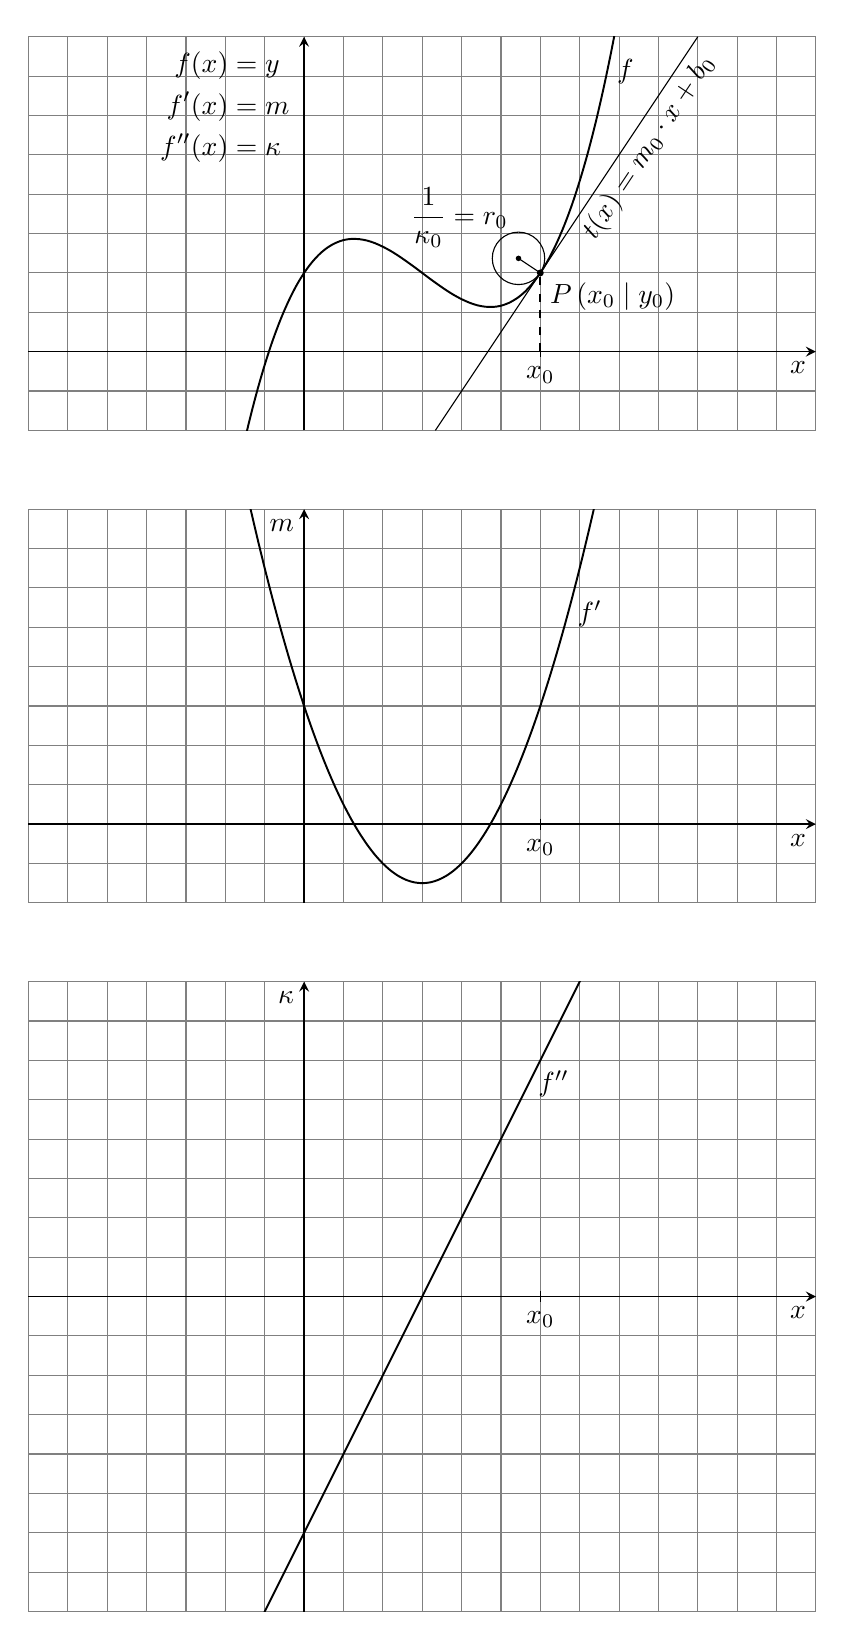
\begin{tikzpicture}[scale=1.000]
    % grid
    \draw[draw=black!50!white] (-5.000, -1.000) grid[step=0.5] (5.000, 4.000);
    % x-axis
    \draw[line width=0.6pt, ->, >=stealth] (-5.000, 0) -- (5.000, 0) node[below left] {$x$};
    % y-axis
    \draw[line width=0.6pt, ->, >=stealth] (-1.5, -1.000) -- (-1.5, 4.000) node[below left]
    {%
      \begin{minipage}{5em}
        \vspace*{-\abovedisplayskip}
        \begin{equation*}
          \begin{split}
            f(x)&=y\\
            f'(x)&=m\\
            f''(x)&=\kappa
          \end{split}
        \end{equation*}
      \end{minipage}%
    };
    \begin{scope}[line width=0.7pt]
      % f(x) = 1/3x^3 - 3/4x + 1
      % xmin =  -5.000
      % xmax =   5.000
      % ymin =  -1.000
      % ymax =   4.000
      % dx   =   0.100
      \clip (-5.000, -1.000) rectangle (5.000, 4.000);
      \draw plot[smooth] coordinates
      {
        ( -5.000,  -4.000) ( -4.900,  -4.000) ( -4.800,  -4.000)
        ( -4.700,  -4.000) ( -4.600,  -4.000) ( -4.500,  -4.000)
        ( -4.400,  -4.000) ( -4.300,  -4.000) ( -4.200,  -4.000)
        ( -4.100,  -4.000) ( -4.000,  -4.000) ( -3.900,  -4.000)
        ( -3.800,  -4.000) ( -3.700,  -4.000) ( -3.600,  -4.000)
        ( -3.500,  -4.000) ( -3.400,  -4.000) ( -3.300,  -4.000)
        ( -3.200,  -4.000) ( -3.100,  -4.000) ( -3.000,  -4.000)
        ( -2.900,  -4.000) ( -2.800,  -4.000) ( -2.700,  -3.536)
        ( -2.600,  -2.909) ( -2.500,  -2.333) ( -2.400,  -1.808)
        ( -2.300,  -1.331) ( -2.200,  -0.899) ( -2.100,  -0.512)
        ( -2.000,  -0.167) ( -1.900,   0.139) ( -1.800,   0.406)
        ( -1.700,   0.637) ( -1.600,   0.835) ( -1.500,   1.000)
        ( -1.400,   1.135) ( -1.300,   1.243) ( -1.200,   1.324)
        ( -1.100,   1.381) ( -1.000,   1.417) ( -0.900,   1.432)
        ( -0.800,   1.429) ( -0.700,   1.411) ( -0.600,   1.378)
        ( -0.500,   1.333) ( -0.400,   1.279) ( -0.300,   1.216)
        ( -0.200,   1.147) ( -0.100,   1.075) (  0.000,   1.000)
        (  0.100,   0.925) (  0.200,   0.853) (  0.300,   0.784)
        (  0.400,   0.721) (  0.500,   0.667) (  0.600,   0.622)
        (  0.700,   0.589) (  0.800,   0.571) (  0.900,   0.568)
        (  1.000,   0.583) (  1.100,   0.619) (  1.200,   0.676)
        (  1.300,   0.757) (  1.400,   0.865) (  1.500,   1.000)
        (  1.600,   1.165) (  1.700,   1.363) (  1.800,   1.594)
        (  1.900,   1.861) (  2.000,   2.167) (  2.100,   2.512)
        (  2.200,   2.899) (  2.300,   3.331) (  2.400,   3.808)
        (  2.500,   4.333) (  2.600,   4.909) (  2.700,   5.536)
        (  2.800,   6.217) (  2.900,   6.955) (  3.000,   7.000)
        (  3.100,   7.000) (  3.200,   7.000) (  3.300,   7.000)
        (  3.400,   7.000) (  3.500,   7.000) (  3.600,   7.000)
        (  3.700,   7.000) (  3.800,   7.000) (  3.900,   7.000)
        (  4.000,   7.000) (  4.100,   7.000) (  4.200,   7.000)
        (  4.300,   7.000) (  4.400,   7.000) (  4.500,   7.000)
        (  4.600,   7.000) (  4.700,   7.000) (  4.800,   7.000)
        (  4.900,   7.000) (  5.000,   7.000)
      };
    \end{scope}
    \begin{scope}
      % f(x)  = 1/3x^3 - 3/4x + 1
      % f'(x) = x^2 - 3/4
      % x0    =   1.500
      % y0    =   1.000
      % t(x)  = 3/2x - 5/4
      \clip (-5.000, -1.000) rectangle (5.000, 4.000);
      \draw (0.167, -1.000) -- (3.500, 4.000);
    \end{scope}
    % t(x) = m0 * x + b
    \node[below=-10pt, rotate=56.310] at (2.500, 2.500)
    {%
      \begin{minipage}{8em}
        \vspace*{-\abovedisplayskip}
        \begin{equation*}
          t(x)=m_0\cdot x+b_0
        \end{equation*}
      \end{minipage}%
    };
    \begin{scope}
      % f(x)   = 1/3x^3 - 3/4x + 1
      % f'(x)  = x^2 - 3/4
      % f''(x) = 2x
      % x0     =   1.500
      % y0     =   1.000
      % kappa  =   3.000
      % r      =   0.333
      % Mx     =   1.223
      % My     =   1.185
      \fill (1.223, 1.185) circle[radius=1.00pt];
      \draw (1.223, 1.185) circle[radius=0.333];
      \draw (1.223, 1.185) -- (1.500, 1.000);
    \end{scope}
    % 1/k0 = r0
    \node[above left=0.333] at (1.223, 1.185)
    {%
      $\displaystyle\frac{1}{\kappa_0}=r_0$%
    };
    % point of contact
    \fill (  1.500,   1.000) circle[radius=1.25pt] node[below right] {$P\left(x_0\;\middle|\;y_0\right)$};
    % x0
    \draw[style=dashed, line width=0.6pt] (1.500, 0) -- (1.500, 1.000);
    \draw (1.500, 2pt) -- (1.500, -2pt) node[below] {$x_0$};
    % f
    \node[right] at (2.350, 3.563) {$f$};
    % f'(x)
    \begin{scope}[yshift=-6.000cm]
      % grid
      \draw[draw=black!50!white] (-5.000, -1.000) grid[step=0.5] (5.000, 4.000);
      % x-axis
      \draw[line width=0.6pt, ->, >=stealth] (-5.000, 0) -- (5.000, 0) node[below left] {$x$};
      % y-axis
      \draw[line width=0.6pt, ->, >=stealth] (-1.5, -1.000) -- (-1.5, 4.000) node[below left] {$m$};
      \begin{scope}[line width=0.7pt]
        % f(x) = x^2 - 3/4
        % xmin =  -5.000
        % xmax =   5.000
        % ymin =  -1.000
        % ymax =   4.000
        % dx   =   0.100
        \clip (-5.000, -1.000) rectangle (5.000, 4.000);
        \draw plot[smooth] coordinates
        {
          ( -5.000,   7.000) ( -4.900,   7.000) ( -4.800,   7.000)
          ( -4.700,   7.000) ( -4.600,   7.000) ( -4.500,   7.000)
          ( -4.400,   7.000) ( -4.300,   7.000) ( -4.200,   7.000)
          ( -4.100,   7.000) ( -4.000,   7.000) ( -3.900,   7.000)
          ( -3.800,   7.000) ( -3.700,   7.000) ( -3.600,   7.000)
          ( -3.500,   7.000) ( -3.400,   7.000) ( -3.300,   7.000)
          ( -3.200,   7.000) ( -3.100,   7.000) ( -3.000,   7.000)
          ( -2.900,   7.000) ( -2.800,   7.000) ( -2.700,   6.540)
          ( -2.600,   6.010) ( -2.500,   5.500) ( -2.400,   5.010)
          ( -2.300,   4.540) ( -2.200,   4.090) ( -2.100,   3.660)
          ( -2.000,   3.250) ( -1.900,   2.860) ( -1.800,   2.490)
          ( -1.700,   2.140) ( -1.600,   1.810) ( -1.500,   1.500)
          ( -1.400,   1.210) ( -1.300,   0.940) ( -1.200,   0.690)
          ( -1.100,   0.460) ( -1.000,   0.250) ( -0.900,   0.060)
          ( -0.800,  -0.110) ( -0.700,  -0.260) ( -0.600,  -0.390)
          ( -0.500,  -0.500) ( -0.400,  -0.590) ( -0.300,  -0.660)
          ( -0.200,  -0.710) ( -0.100,  -0.740) (  0.000,  -0.750)
          (  0.100,  -0.740) (  0.200,  -0.710) (  0.300,  -0.660)
          (  0.400,  -0.590) (  0.500,  -0.500) (  0.600,  -0.390)
          (  0.700,  -0.260) (  0.800,  -0.110) (  0.900,   0.060)
          (  1.000,   0.250) (  1.100,   0.460) (  1.200,   0.690)
          (  1.300,   0.940) (  1.400,   1.210) (  1.500,   1.500)
          (  1.600,   1.810) (  1.700,   2.140) (  1.800,   2.490)
          (  1.900,   2.860) (  2.000,   3.250) (  2.100,   3.660)
          (  2.200,   4.090) (  2.300,   4.540) (  2.400,   5.010)
          (  2.500,   5.500) (  2.600,   6.010) (  2.700,   6.540)
          (  2.800,   7.000) (  2.900,   7.000) (  3.000,   7.000)
          (  3.100,   7.000) (  3.200,   7.000) (  3.300,   7.000)
          (  3.400,   7.000) (  3.500,   7.000) (  3.600,   7.000)
          (  3.700,   7.000) (  3.800,   7.000) (  3.900,   7.000)
          (  4.000,   7.000) (  4.100,   7.000) (  4.200,   7.000)
          (  4.300,   7.000) (  4.400,   7.000) (  4.500,   7.000)
          (  4.600,   7.000) (  4.700,   7.000) (  4.800,   7.000)
          (  4.900,   7.000) (  5.000,   7.000)
        };
      \end{scope}
      % f'
      \node[right] at (1.850, 2.673) {$f'$};
      % x0
      \draw (1.500, 2pt) -- (1.500, -2pt) node[below] {$x_0$};
    \end{scope}
    % f''(x)
    \begin{scope}[yshift=-12.000cm]
      % grid
      \draw[draw=black!50!white] (-5.000, -4.000) grid[step=0.5] (5.000, 4.000);
      % x-axis
      \draw[line width=0.6pt, ->, >=stealth] (-5.000, 0) -- (5.000, 0) node[below left] {$x$};
      % y-axis
      \draw[line width=0.6pt, ->, >=stealth] (-1.5, -4.000) -- (-1.5, 4.000) node[below left] {$\kappa$};
      \begin{scope}[line width=0.7pt]
        % f(x) = 2x
        % xmin =  -5.000
        % xmax =   5.000
        % ymin =  -4.000
        % ymax =   4.000
        % dx   =   0.100
        \clip (-5.000, -4.000) rectangle (5.000, 4.000);
        \draw plot[smooth] coordinates
        {
          ( -5.000,  -7.000) ( -4.900,  -7.000) ( -4.800,  -7.000)
          ( -4.700,  -7.000) ( -4.600,  -7.000) ( -4.500,  -7.000)
          ( -4.400,  -7.000) ( -4.300,  -7.000) ( -4.200,  -7.000)
          ( -4.100,  -7.000) ( -4.000,  -7.000) ( -3.900,  -7.000)
          ( -3.800,  -7.000) ( -3.700,  -7.000) ( -3.600,  -7.000)
          ( -3.500,  -7.000) ( -3.400,  -6.800) ( -3.300,  -6.600)
          ( -3.200,  -6.400) ( -3.100,  -6.200) ( -3.000,  -6.000)
          ( -2.900,  -5.800) ( -2.800,  -5.600) ( -2.700,  -5.400)
          ( -2.600,  -5.200) ( -2.500,  -5.000) ( -2.400,  -4.800)
          ( -2.300,  -4.600) ( -2.200,  -4.400) ( -2.100,  -4.200)
          ( -2.000,  -4.000) ( -1.900,  -3.800) ( -1.800,  -3.600)
          ( -1.700,  -3.400) ( -1.600,  -3.200) ( -1.500,  -3.000)
          ( -1.400,  -2.800) ( -1.300,  -2.600) ( -1.200,  -2.400)
          ( -1.100,  -2.200) ( -1.000,  -2.000) ( -0.900,  -1.800)
          ( -0.800,  -1.600) ( -0.700,  -1.400) ( -0.600,  -1.200)
          ( -0.500,  -1.000) ( -0.400,  -0.800) ( -0.300,  -0.600)
          ( -0.200,  -0.400) ( -0.100,  -0.200) (  0.000,   0.000)
          (  0.100,   0.200) (  0.200,   0.400) (  0.300,   0.600)
          (  0.400,   0.800) (  0.500,   1.000) (  0.600,   1.200)
          (  0.700,   1.400) (  0.800,   1.600) (  0.900,   1.800)
          (  1.000,   2.000) (  1.100,   2.200) (  1.200,   2.400)
          (  1.300,   2.600) (  1.400,   2.800) (  1.500,   3.000)
          (  1.600,   3.200) (  1.700,   3.400) (  1.800,   3.600)
          (  1.900,   3.800) (  2.000,   4.000) (  2.100,   4.200)
          (  2.200,   4.400) (  2.300,   4.600) (  2.400,   4.800)
          (  2.500,   5.000) (  2.600,   5.200) (  2.700,   5.400)
          (  2.800,   5.600) (  2.900,   5.800) (  3.000,   6.000)
          (  3.100,   6.200) (  3.200,   6.400) (  3.300,   6.600)
          (  3.400,   6.800) (  3.500,   7.000) (  3.600,   7.000)
          (  3.700,   7.000) (  3.800,   7.000) (  3.900,   7.000)
          (  4.000,   7.000) (  4.100,   7.000) (  4.200,   7.000)
          (  4.300,   7.000) (  4.400,   7.000) (  4.500,   7.000)
          (  4.600,   7.000) (  4.700,   7.000) (  4.800,   7.000)
          (  4.900,   7.000) (  5.000,   7.000)
        };
      \end{scope}
      % f''
      \node[right] at (1.350, 2.700) {$f''$};
      % x0
      \draw (1.500, 2pt) -- (1.500, -2pt) node[below] {$x_0$};
    \end{scope}
  \end{tikzpicture}
\end{center}

% ------------------------------------------------------------------------------
\end{document}
% ------------------------------------------------------------------------------

